\documentclass[a4paper,12pt]{article} 

% First, we usually want to set the margins of our document. For this we use the package geometry.
\usepackage[top = 2.5cm, bottom = 2.5cm, left = 2.5cm, right = 2.5cm]{geometry} 
\usepackage[T1]{fontenc}
\usepackage[utf8]{inputenc}

% The following two packages - multirow and booktabs - are needed to create nice looking tables.
\usepackage{multirow} % Multirow is for tables with multiple rows within one cell.
\usepackage{booktabs} % For even nicer tables.

% As we usually want to include some plots (.pdf files) we need a package for that.
\usepackage{graphicx} 

% The default setting of LaTeX is to indent new paragraphs. This is useful for articles. But not really nice for homework problem sets. The following command sets the indent to 0.
\usepackage{setspace}
\setlength{\parindent}{0in}

% Package to place figures where you want them.
\usepackage{float}

% The fancyhdr package let's us create nice headers.
\usepackage{fancyhdr}

\usepackage{amsmath,amsthm,caption}
\usepackage[open]{bookmark}
\usepackage{minted}


% To make our document nice we want a header and number the pages in the footer.

\pagestyle{fancy} % With this command we can customize the header style.

\fancyhf{} % This makes sure we do not have other information in our header or footer.

\lhead{\footnotesize Computer Network: Assignment 2}% \lhead puts text in the top left corner. \footnotesize sets our font to a smaller size.

%\rhead works just like \lhead (you can also use \chead)
\rhead{\footnotesize Mengxuan Wu} %<---- Fill in your lastnames.

% Similar commands work for the footer (\lfoot, \cfoot and \rfoot).
% We want to put our page number in the center.
\cfoot{\footnotesize \thepage} 

\begin{document}

\thispagestyle{empty} % This command disables the header on the first page. 

\begin{tabular}{p{15.5cm}}
{\large \bf Computer Network} \\
Southern University of Science and Technology \\ Mengxuan Wu \\ 12212006 \\
\hline
\\
\end{tabular}

\vspace*{0.3cm} %add some vertical space in between the line and our title.

\begin{center}
	{\Large \bf Theory Assignment 2}
	\vspace{2mm}

	{\bf Mengxuan Wu}
		
\end{center}  

\vspace{0.4cm}

\section*{Question 1}

\subsection*{(a)}

To compute the checksum, we first add each 16-bit word into 
\begin{equation*}
  1001100110011111 + 1010101010101010 = 1\_0100010001001001
\end{equation*}

Then we add the carry to the result
\begin{equation*}
  1 + 0100010001001001 = 0100010001001010
\end{equation*}

Finally, we take the one's complement of the result
\begin{equation*}
  1011101110110101
\end{equation*}

\subsection*{(b)}

To check whether the data is corrupted, the receiver needs to compute the checksum of the received data. Similarly, we first add each 16-bit word and add the carry to the result. Then we take the one's complement of the result. If the checksum is 16 1's, the data is not corrupted. Otherwise, the data is corrupted.

\subsection*{(c)}

Even if the checksum detects no errors, the data may still be corrupted. The data may experience multiple bit errors that cancel each other out. 

For example, if the data is 0000 0000 0000 0000, then its checksum is 1111 1111 1111 1111. Suppose during transmission, the data and checksum's last bit are both flipped. Then, the data becomes 0000 0000 0000 0001, and its checksum is 1111 1111 1111 1110. However, summation of the data and the checksum is still 1111 1111 1111 1111, which indicates no error.

\section*{Question 2}

Firstly, go-back-N's receiving window is always one frame, while selective repeat's receiving window can be multiple frames. 

Secondly, go-back-N retransmits all frames from the lost frame to the last frame received correctly. In contrast, selective repeat only retransmits the lost frame.

Thirdly, go-back-N has a cumulative acknowledgment, which means the receiver only sends one acknowledgment for the last frame received correctly. In contrast, selective repeat has individual acknowledgment, which means the receiver sends an acknowledgment for each frame received correctly.

\section*{Question 3}

\begin{figure}[H]
  \centering
  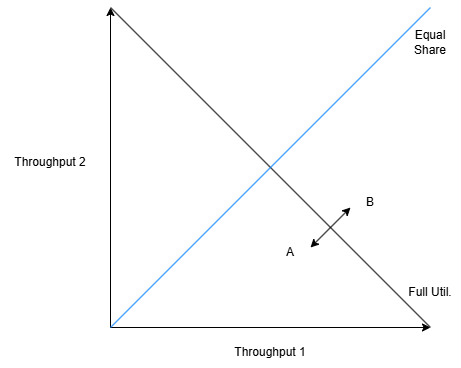
\includegraphics[width=0.8\textwidth]{figure/AIAD.drawio.png}
\end{figure}

No, AIAD will not converge to equal share of bandwidth. 

As demonstrated in the figure, the two connection will fluctuate between A and B. At point A, the two connections will increase their window size, which reaches point B. At point B, congestion occurs, and the two connections will decrease their window size, which reaches point A. The two connections will keep fluctuating between A and B, and the bandwidth will not be equally shared.

\section*{Question 4}

\subsection*{(a)}

102

\subsection*{(b)}

110

\subsection*{(c)}

110

\subsection*{(d)}

130

\subsection*{(e)}

102

\subsection*{(f)}

130

\section*{Question 5}

In congestion avoidance state, the sender increases the window size by 1 MSS every RTT. Thus, the time to increase window size from 8KB to 32KB is
\begin{equation*}
  \frac{32 \text{KB} - 8 \text{KB}}{2 \text{KB / RTT}} \times 4 \text{ms / RTT} = 48 \text{ms}
\end{equation*}

\section*{Question 6}

\begin{table}[H]
  \centering
  \begin{tabular}{ccc}
    \toprule
    Prefix & Range of destination host addresses & Number of addresses \\
    \midrule
    1110**** & 11100100 - 11101111 & 12 \\
    111000** & 11100000 - 11100011 & 4 \\
    111111** & 11111100 - 11111111 & 4 \\
    Otherwise & 00000000 - 11011111 and 11110000 - 11111011 & 236 \\
    \bottomrule
  \end{tabular}
\end{table}

\section*{Question 7}

Since we allocate IP address group with size of power of 2, each of the 4 groups will have 64 addresses.

Thus, the prefixes are
\begin{itemize}
  \item Organization 1: 128.119.40.0/26
  \item Organization 2: 128.119.40.64/26
  \item Organization 3: 128.119.40.128/26
  \item Organization 4: 128.119.40.192/26
\end{itemize}

\section*{Question 8}

\subsection*{a)}

Without poisoned reverse, the distance vector table of node $Z$ is
\begin{table}[H]
  \centering
  \begin{tabular}{ccccc}
    \toprule
    \multirow{2}{*}{From} & \multicolumn{4}{c}{Cost To} \\
    \cmidrule{2-5}
    & $X$ & $Y$ & $Z$ & $W$ \\
    \midrule
    $X$ & 0 & 3 & 1 & 13 \\
    $Y$ & 3 & 0 & 2 & 10 \\
    $Z$ & 1 & 2 & 0 & 12 \\
    \bottomrule
  \end{tabular}
\end{table}

\subsection*{b)}

With poisoned reverse, the distance vector table of node $Z$ is
\begin{table}[H]
  \centering
  \begin{tabular}{ccccc}
    \toprule
    \multirow{2}{*}{From} & \multicolumn{4}{c}{Cost To} \\
    \cmidrule{2-5}
    & $X$ & $Y$ & $Z$ & $W$ \\
    \midrule
    $X$ & 0 & $\infty$ & 1 & $\infty$ \\
    $Y$ & $\infty$ & 0 & 2 & 10 \\
    $Z$ & 1 & 2 & 0 & 12 \\
    \bottomrule
  \end{tabular}
\end{table}

\subsection*{c)}

\begin{table}[H]
  \centering
  \begin{tabular}{cc}
    \toprule
    Prefix & Interface \\
    \midrule
    176.14.255.0/25 & $(Z, Y)$ \\
    176.14.255.128/25 & $(Z, Y)$ \\
    \bottomrule
  \end{tabular}
\end{table}

\subsection*{d)}

Yes, the two entries can be combined into one entry with prefix
\begin{table}[H]
  \centering
  \begin{tabular}{cc}
    \toprule
    Prefix & Interface \\
    \midrule
    176.14.255.0/24 & $(Z, Y)$ \\
    \bottomrule
  \end{tabular}
\end{table}

\subsection*{e)}

\subsubsection*{(i)}

When cost of link $(Y, Z)$ increases to 100, node $Y$ and $Z$ will update their distance vector table immediately. 

\subsubsection*{(ii)}

In the first iteration, node $Z$ discovers that the cost to $Y$ is 100, and updates its distance vector table. The distance vector table of node $Z$ is

\begin{table}[H]
  \centering
  \begin{tabular}{ccccc}
    \toprule
    \multirow{2}{*}{From} & \multicolumn{4}{c}{Cost To} \\
    \cmidrule{2-5}
    & $X$ & $Y$ & $Z$ & $W$ \\
    \midrule
    $X$ & 0 & 3 & 1 & 13 \\
    $Y$ & 3 & 0 & 2 & 10 \\
    $Z$ & 1 & 4 & 0 & 12 \\
    \bottomrule
  \end{tabular}
\end{table}

\subsubsection*{(iii)}

The updates of the distance vector table of node $X$ and $Z$ can be viewed as
\begin{align*}
  D_Z(Y) &= \min\{c(Z, X) + D_X(Y), c(Z, Y)\} = \min\{1 + D_X(Y), 100\} \\
  D_X(Y) &= \min\{c(X, Z) + D_Z(Y), c(X, Y)\} = \min\{1 + D_Z(Y), 30\}
\end{align*}

Thus, the two values' update depends on each other, and the two nodes will keep updating the values until they reach the true cost by adding 1 each iteration.
\begin{align*}
  D_Z(Y) &= \min\{1 + 3, 100\} = 4 \\
  D_X(Y) &= \min\{1 + 4, 30\} = 5 \\
  D_Z(Y) &= \min\{1 + 5, 100\} = 6 \\
  D_X(Y) &= \min\{1 + 6, 30\} = 7 \\
  &\vdots \\
  D_Z(Y) &= \min\{1 + 30, 100\} = 31 \\
\end{align*}

Thus, $Z$ needs 27 iterations to discover the true cost (from 4 to 31). This example explains ``bad news travels slowly''.

\end{document}